\documentclass[12pt]{article}

\usepackage{graphicx}% Include figure files
\usepackage{dcolumn}% Align table columns on decimal point

% Use Arial font %
\usepackage{helvet}
\renewcommand{\familydefault}{\sfdefault} 

% Default margins and paper properties %
\usepackage[a4, portrait, margin=0.6in]{geometry}

\begin{document}
	\title{Hypothesis plots summary} % Force line breaks with \\
	\author{1666957, Gustavo Espinal Lugo}
	\date{\today} % It is always \today, today, %  but any date may be explicitly specified

	\maketitle
	%\tableofcontents
	
	\section*{Plots and corresponding metadata}
	mean expected W mass: 80.379 $[GeV/c^{2}]$,\\
mean hypothesis masses: [78.  78.5 79.  79.5 80.  80.5 81.  81.5 82. ] $[GeV/c^{2}]$,\\
mass width: 2.07 $[GeV/c^{2}]$,\\
chi\_square value of hypothesis fit: 54.43375760081301\\
	Absolute path to figure: /home/physics/phuxdp/Desktop/PX402 Physics Project/WBosonProject/T2W5/plots/muPT\_80.379\_2.07\_between\_78\_and\_82\_summary.png\\
	Next lines are the data of the shown histograms (if needed): \\
	All quantities: 	80.379, [78.  78.5 79.  79.5 80.  80.5 81.  81.5 82. ], 2070, 54.43375760081301\\
	X\_energ\_vls = [0.6, 1.7999999999999998, 3.0, 4.199999999999999, 5.4, 6.6, 7.8, 9.0, 10.2, 11.399999999999999, 12.6, 13.799999999999999, 15.0, 16.2, 17.4, 18.6, 19.799999999999997, 21.0, 22.2, 23.4, 24.6, 25.799999999999997, 27.0, 28.199999999999996, 29.4, 30.6, 31.799999999999997, 33.0, 34.2, 35.4, 36.599999999999994, 37.8, 39.0, 40.2, 41.4, 42.599999999999994, 43.8, 45.0, 46.2, 47.4, 48.599999999999994, 49.8, 51.0, 52.2, 53.4, 54.599999999999994, 55.8, 57.0, 58.199999999999996, 59.4, 60.599999999999994, 61.8, 63.0, 64.19999999999999, 65.4, 66.6, 67.8, 69.0, 70.19999999999999, 71.4, 72.6, 73.8, 75.0, 76.19999999999999, 77.4, 78.6, 79.8, 81.0, 82.19999999999999, 83.4, 84.6, 85.8, 87.0, 88.19999999999999, 89.4, 90.6, 91.8, 93.0, 94.19999999999999, 95.4, 96.6, 97.8, 99.0, 100.19999999999999, 101.4, 102.6, 103.8, 105.0, 106.19999999999999, 107.4, 108.6, 109.8, 111.0, 112.19999999999999, 113.4, 114.6, 115.79999999999998, 117.0, 118.19999999999999, 119.4]\\
	Y\_data\_bin\_cnts = [0.0, 0.0, 0.0, 0.0, 0.0, 0.0, 0.0, 0.0, 0.0, 0.0, 0.0, 0.0, 0.0, 0.0, 0.0, 2.0, 2.0, 26.0, 1877.0, 93470.0, 122149.0, 130185.0, 139392.0, 148542.0, 157370.0, 166200.0, 175733.0, 185306.0, 194236.0, 202199.0, 209770.0, 210468.0, 200967.0, 173994.0, 135804.0, 100636.0, 75854.0, 58474.0, 45997.0, 37262.0, 30356.0, 24933.0, 20658.0, 17367.0, 14853.0, 12565.0, 10682.0, 9134.0, 8082.0, 7030.0, 6114.0, 5301.0, 4651.0, 4168.0, 3705.0, 3289.0, 2962.0, 2612.0, 2332.0, 2129.0, 1953.0, 1793.0, 1574.0, 1392.0, 1286.0, 1180.0, 1045.0, 956.0, 890.0, 814.0, 778.0, 693.0, 593.0, 622.0, 528.0, 518.0, 506.0, 451.0, 404.0, 370.0, 326.0, 337.0, 295.0, 261.0, 247.0, 226.0, 232.0, 212.0, 205.0, 173.0, 155.0, 146.0, 134.0, 133.0, 132.0, 104.0, 114.0, 115.0, 100.0, 85.0]\\
	Y\_model\_bin\_cnts = [0.0, 0.0, 0.0, 0.0, 0.0, 0.0, 0.0, 0.0, 0.9608225226402283, 1.921647071838379, 0.0, 0.0, 0.0, 0.0, 0.9608226418495178, 3.843290328979492, 3.8432936668395996, 26.90304183959961, 1791.922607421875, 90206.78125, 116579.7109375, 126073.7734375, 133806.125, 142110.703125, 151180.640625, 159975.125, 169458.71875, 177724.21875, 185457.875, 194505.890625, 200279.921875, 201648.609375, 192689.234375, 166719.4375, 129773.3828125, 97057.296875, 72612.96875, 56565.30859375, 44595.875, 35620.7109375, 29020.986328125, 23888.619140625, 20124.62109375, 16671.015625, 13836.2490234375, 12109.4482421875, 10349.0107421875, 8852.8359375, 7528.666015625, 6789.70556640625, 5751.892578125, 5217.61767578125, 4541.115234375, 4088.51171875, 3549.4306640625, 3102.599609375, 2816.243408203125, 2506.823974609375, 2319.442138671875, 2040.7733154296875, 1829.393798828125, 1642.9959716796875, 1553.639892578125, 1351.8687744140625, 1265.3953857421875, 1087.64453125, 1001.1709594726562, 963.69921875, 861.852783203125, 833.989013671875, 724.4562377929688, 619.7273559570312, 575.52978515625, 518.8416137695312, 551.5093383789062, 490.0170593261719, 424.68182373046875, 391.0530700683594, 410.26959228515625, 328.6000061035156, 282.48095703125, 306.50140380859375, 283.4420471191406, 268.06878662109375, 248.8524932861328, 211.38050842285156, 214.26296997070312, 196.96827697753906, 182.5560760498047, 162.37884521484375, 160.457275390625, 140.27999877929688, 125.86770629882812, 150.84902954101562, 108.57294464111328, 118.18119049072266, 119.14203643798828, 106.65130615234375, 92.23898315429688, 74.94416046142578]\\

    Found optimal massses ($\chi^2$ roots): [80.40684652] $[GeV/c^{2}]$
    Uncertainty [GeV/c^2]: 0.1807004941410213

	\begin{figure}[tb]
		\centering
		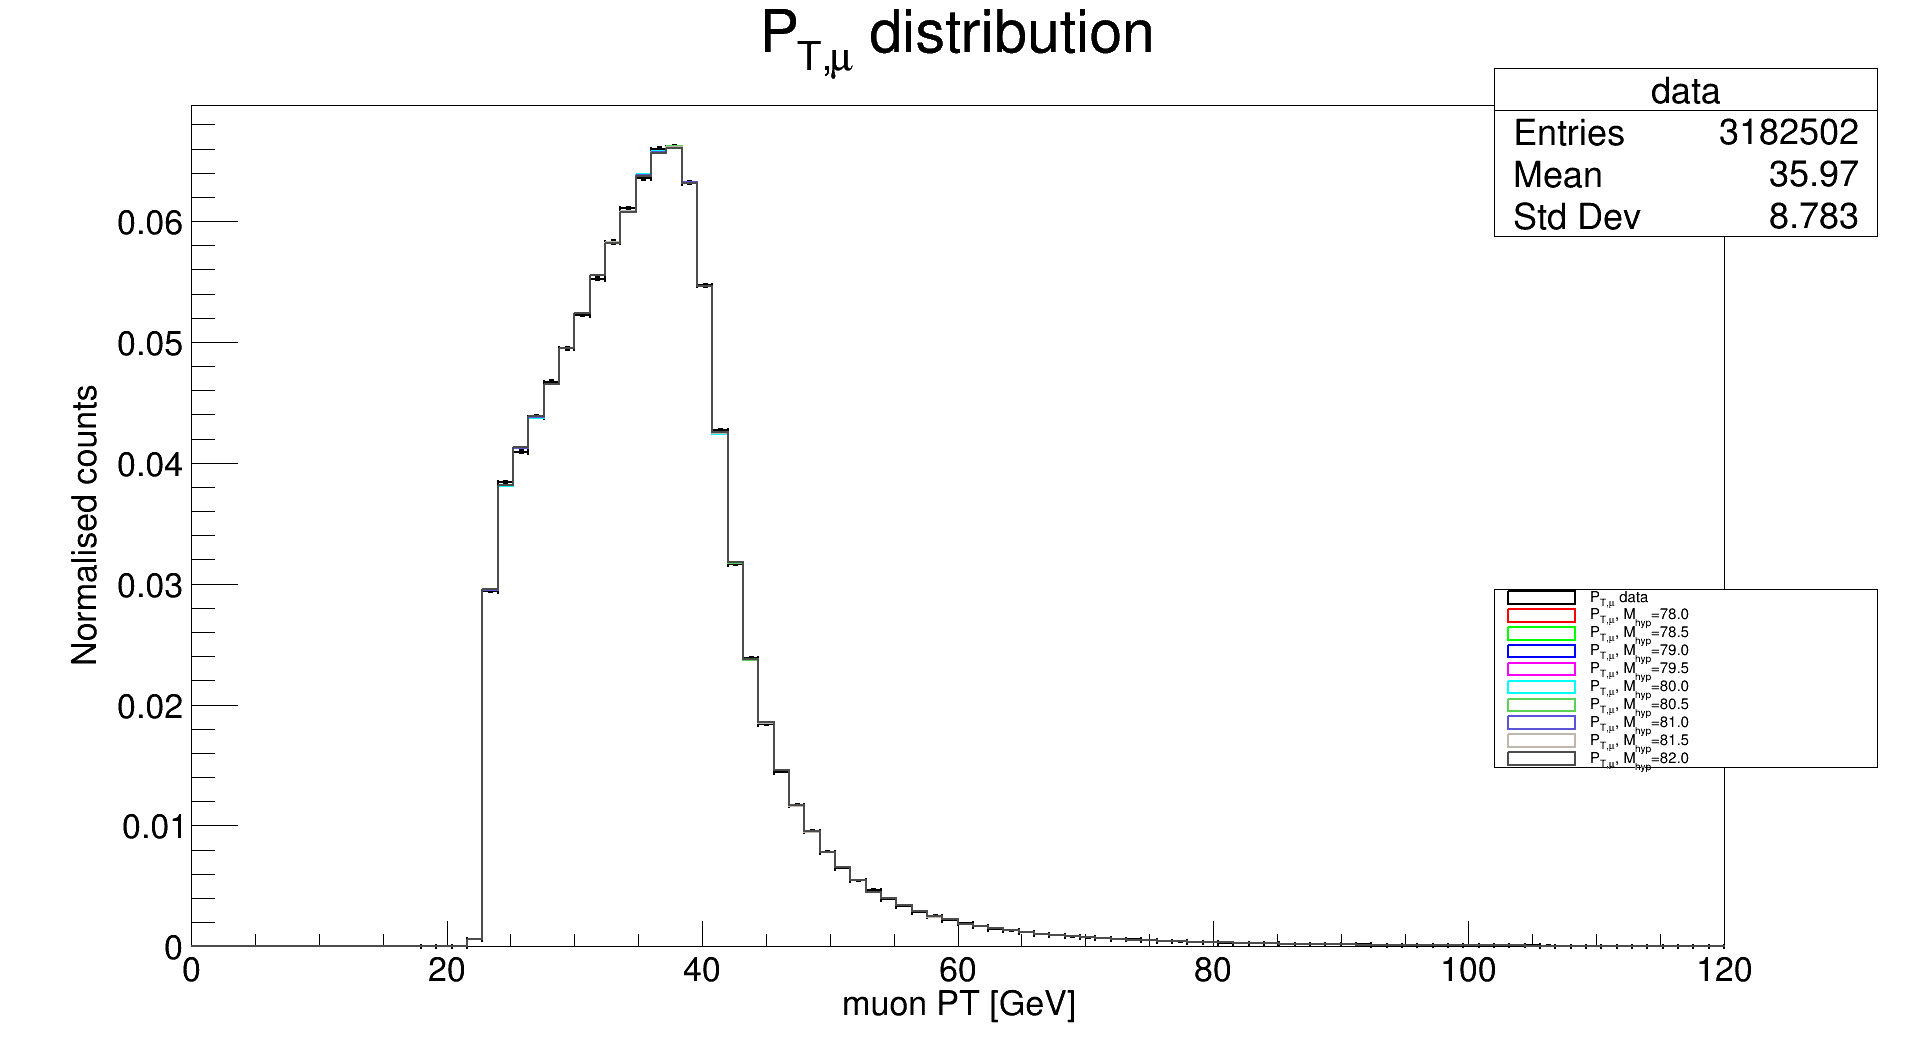
\includegraphics[width=\columnwidth]{/home/physics/phuxdp/Desktop/PX402 Physics Project/WBosonProject/T2W5/plots/muPT_80.379_2.07_between_78_and_82_summary.png}
		\caption{\small Hypothesis masses mean expected W mass: 80.379 $[GeV/c^{2}]$,\\
mean hypothesis masses: [78.  78.5 79.  79.5 80.  80.5 81.  81.5 82. ] $[GeV/c^{2}]$,\\
mass width: 2.07 $[GeV/c^{2}]$,\\
chi_square value of hypothesis fit: 54.43375760081301. }
		\label{fig: fig_0}
	\end{figure}

       \begin{figure}[tb]
		\centering
		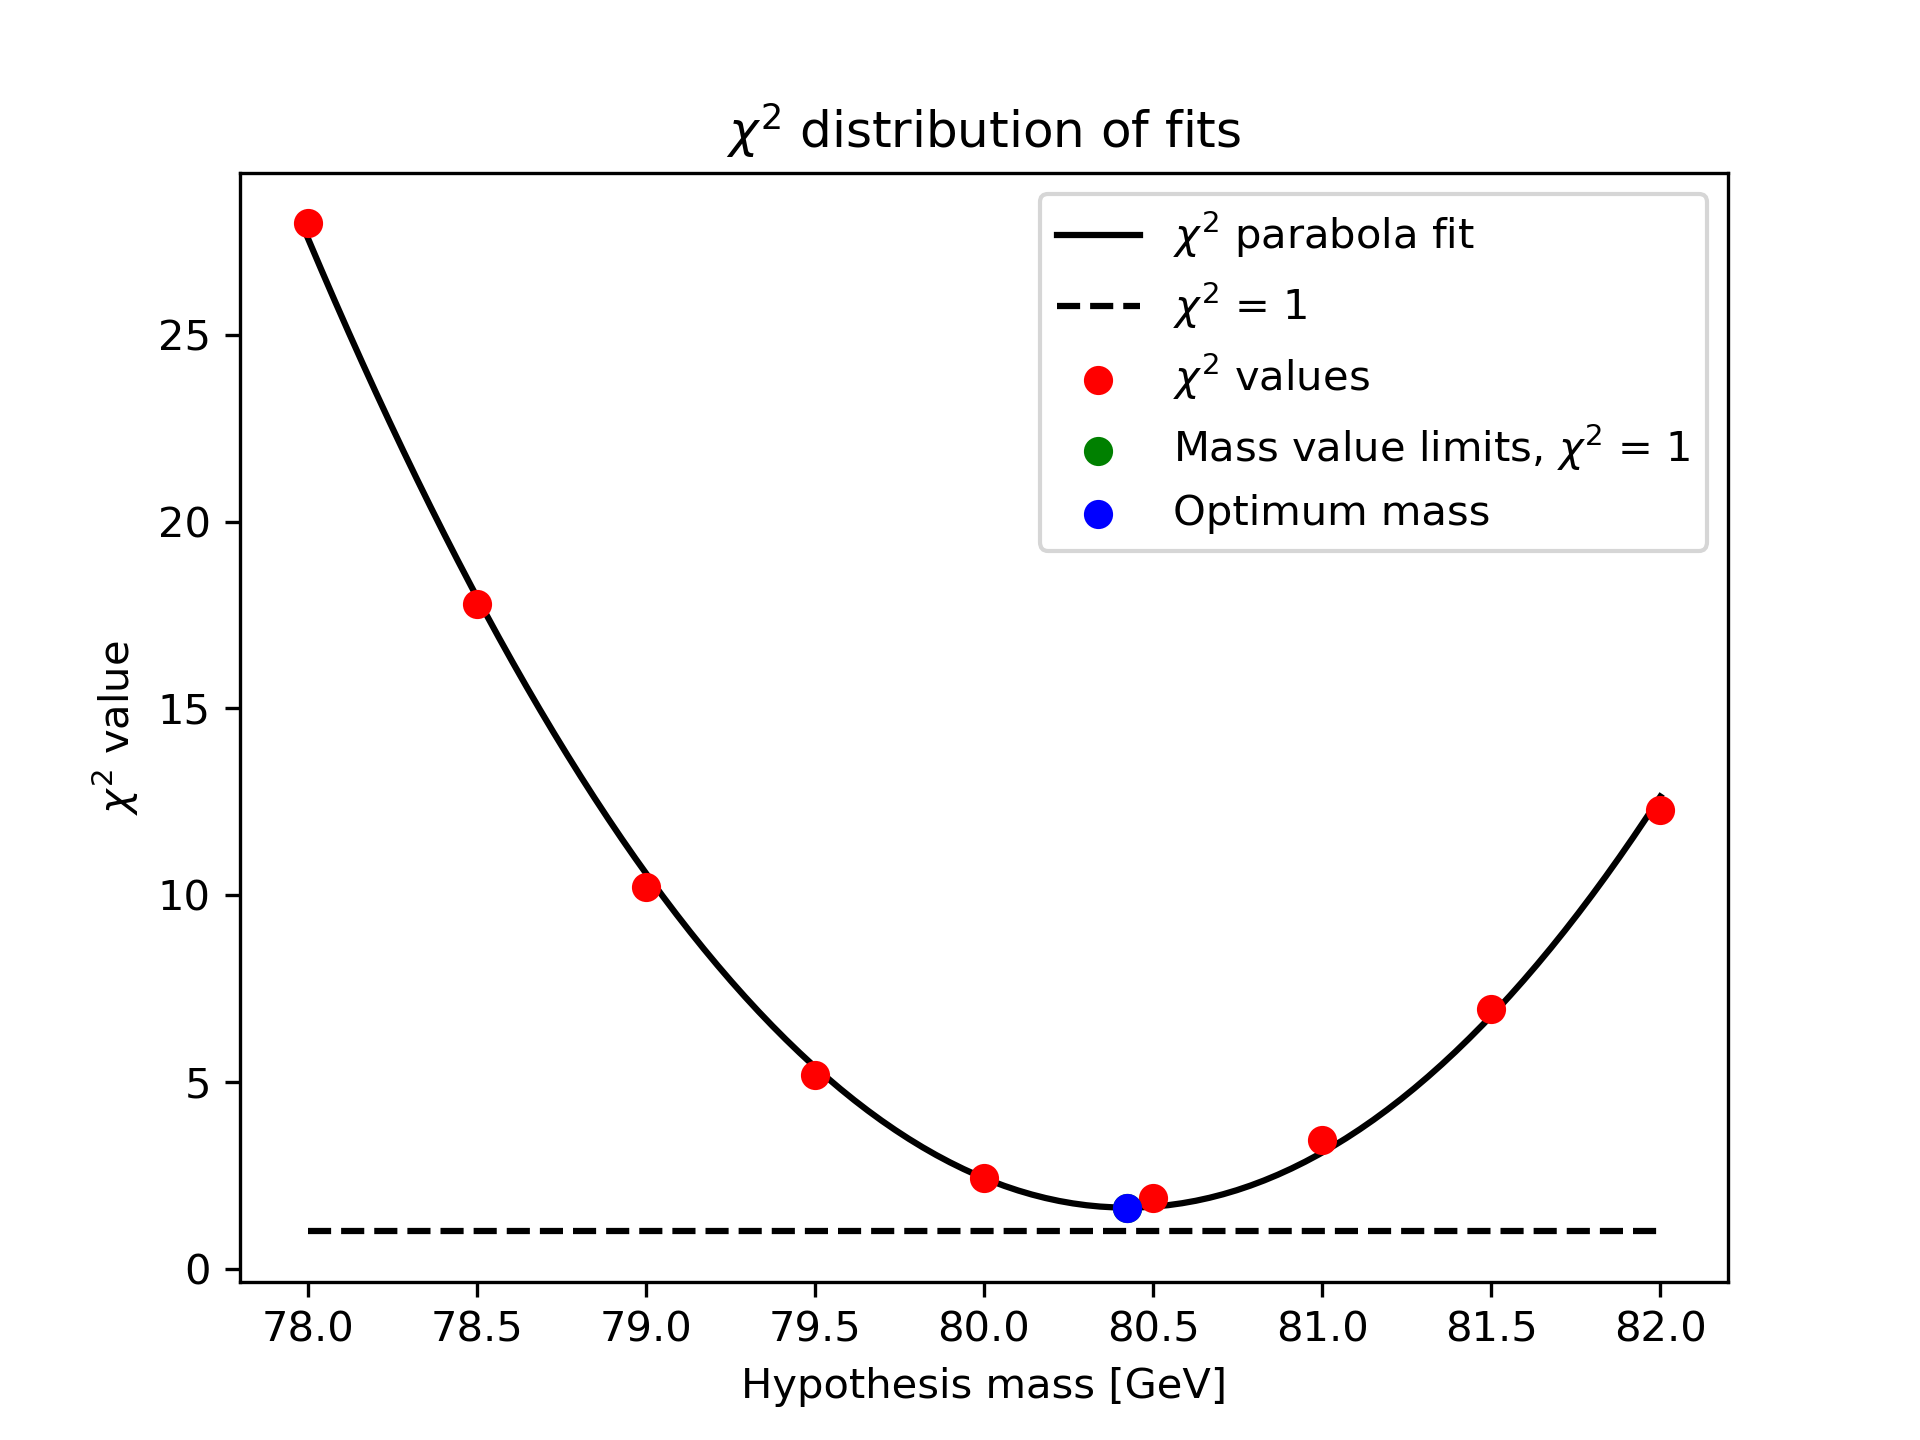
\includegraphics[width=\columnwidth]{/home/physics/phuxdp/Desktop/PX402 Physics Project/WBosonProject/T2W5/plots/chi_square_fits_muPT_80.379_2.07_between_78_and_82_summary.png}
		\caption{\small $\chi^2$ of hypothesis masses. }
		\label{fig: fig_chi_square}
	\end{figure}

    \begin{figure}[tb]
		\centering
		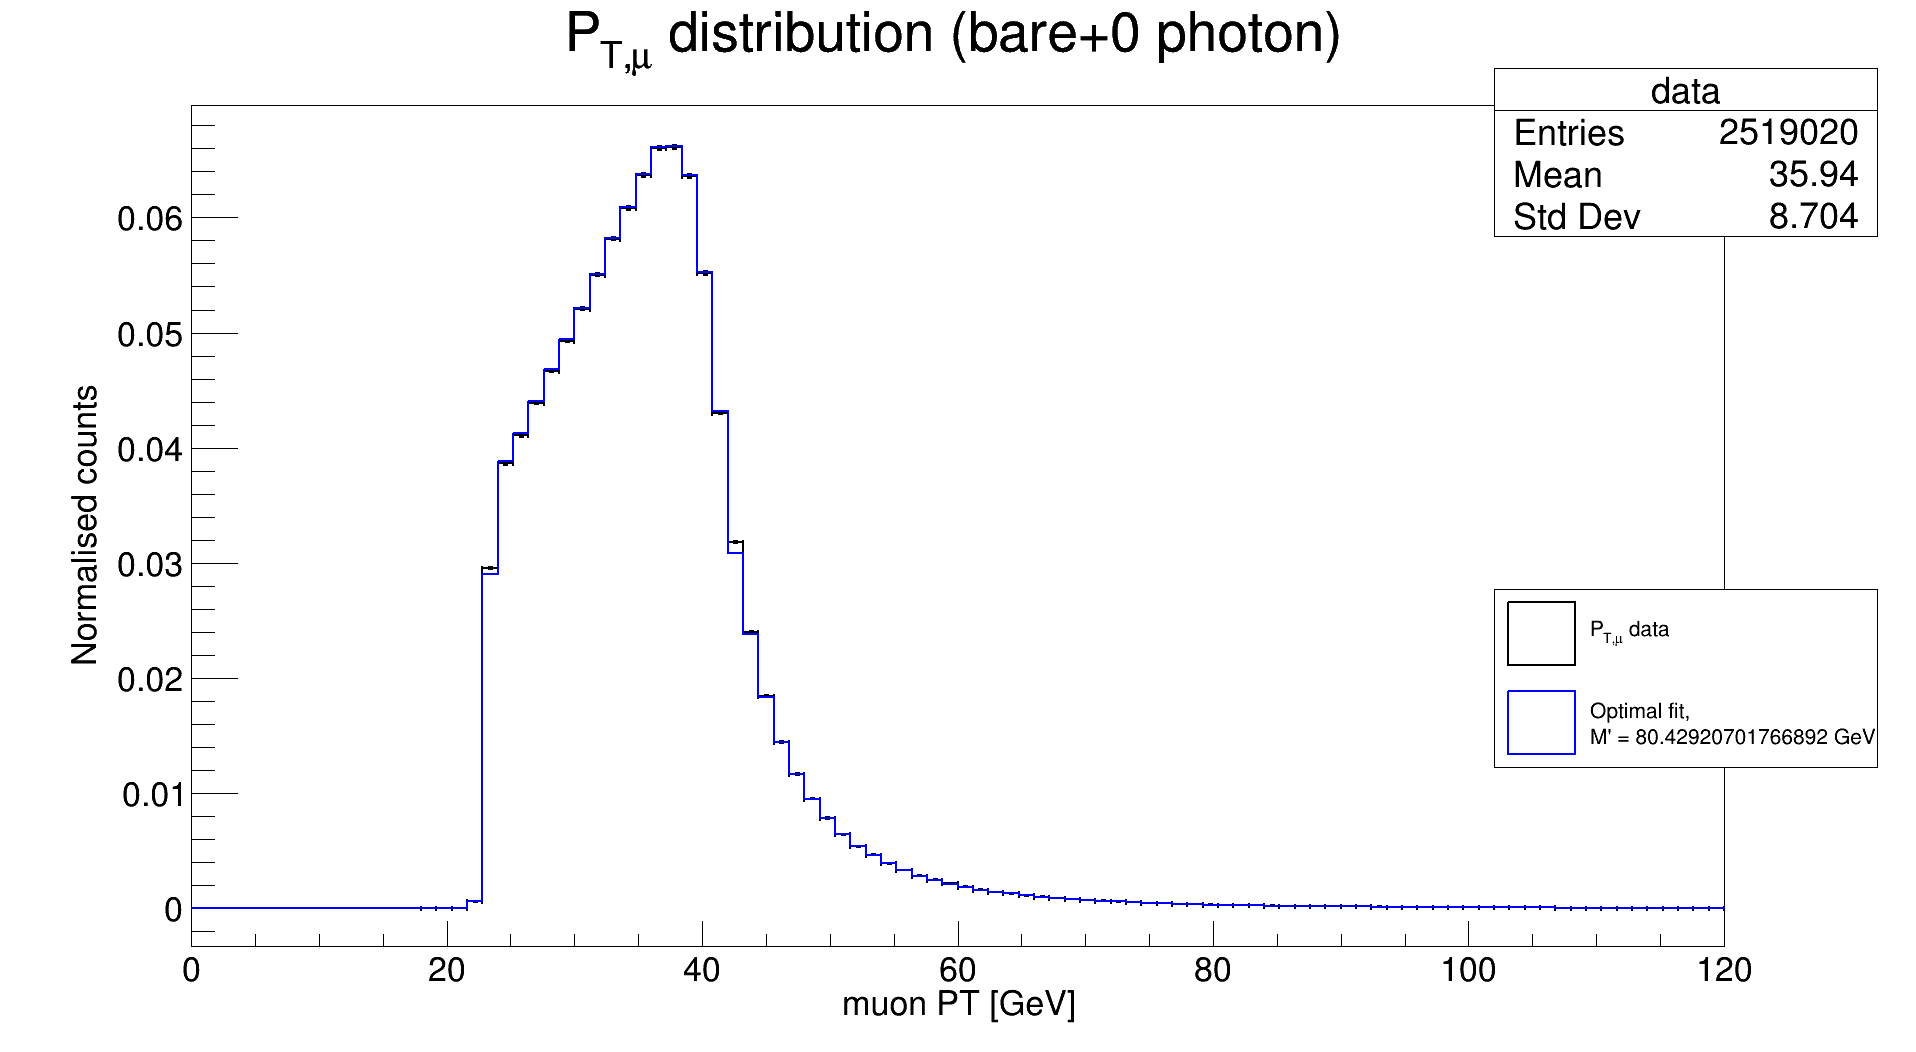
\includegraphics[width=\columnwidth]{/home/physics/phuxdp/Desktop/PX402 Physics Project/WBosonProject/T2W5/plots/optimum_muPT_80.379_2.07_between_78_and_82_summary.png}
		\caption{\small Data and optimum fit with $\chi^2 = 0.14939319155542216$. Used the hypothesis mass of 80.4068465171209$\pm$0.1807004941410213 $[GeV/c^{2}]$. }
		\label{fig: fig_optim_parms}
	\end{figure}
    
\end{document}